The diagram shown in figure \ref{fig:diagramSystem} illustrates the system functionality: recognize voice commands and convert to text, extract the information from text and map to corresponding robot actions (figure \ref{fig:diagramSystem}). 
\begin{figure}[tb]
\centering
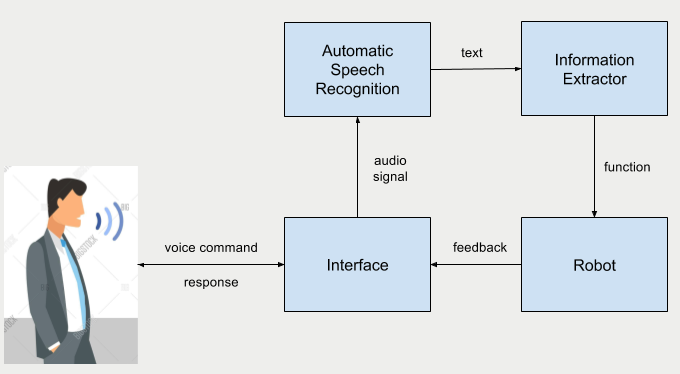
\includegraphics[width = 0.7\hsize]{./figures/diagramSystem}
\caption{Diagram of the system}
\label{fig:diagramSystem}
\end{figure}

Our robot's actions are focused on movement and visual recognition: the robot not also moves according to our commands but also tells us what it sees in its surrounding environment.  

To achieve that, we will solve the problems one by one: 
\begin{enumerate}
	\item meet the Cozmo robot and get familiar with its SDK (section \ref{sec:Cozmo})
	\item build and embed a speech recognizer (section \ref{sec:ASR})
	\item implement and embed an information extractor (section \ref{sec:InfoExt})
	\item explore deep neural network algorithms for visual recognition: 
	\begin{itemize}
		\item train and embed the image classifier (section \ref{sec:imgClass})
		\item train and embed the object detector (section \ref{sec:objDetect})
		\item estimate distance from object to camera (section \ref{sec:camModel})
	\end{itemize}
	\item build our own image dataset from ImageNet (section \ref{sec:dataset}) and play with data preprocessing and augmentation (section \ref{sec:dataPrepAug})
	\item train the image classifier and the object detector using our dataset
	\item transfer learning (section \ref{sec:transferLearning}), fine-tune deep neural networks (subsection \ref{sec:transLearnEval})
	\item deploy object detector server on a workstation in Huxley lab (section \ref{sec:socketConnect}), implement a GUI, and use threads to do event and signal driven programming (section \ref{sec:threading})
	\item set up an experiment to estimate distance between the robot and the object
	\item contribute and share works, ideas and thoughts in open-source community through Github platform (section \ref{sec:github})	
\end{enumerate} 

We will also evaluate our system to see how robust it is in section \ref{sec:imgClasEval} and \ref{sec:objDetEval}. Briefly, our image classifier achieves $> 93\%$ accuracy (comparable to human beings) and decent state-of-the-art object detector which takes only $\approx 0.4$ second to detect and localize objects in an image. This makes our system nearly real-time.


%Two closely related reasons for this booming era of voice-based system is the success of Deep Neural Network along with the availibility of Big Data. 
%
%Deep Neural Network (DNN) is a machine learning method that was introduced in second half of 20th century. Because of its massive computation demand, DNN was not successful until 2012, when strong GPU and big data are available. Previously, traditional methods of speech recognition and speech synthesis based on Gaussian Mixture and Hidden Markov models involve many non-uniform internal-handcrafting rules 
%
%have been taken over by DNN